\chapter{优化设计与实现}
\label{cha:imple}

\section{开放通道SSD访问}

传统SSD的访问方式如图\ref{fig:imple_traditional_ssd}所示。用户态程序发出的文件操作请求经内核的虚拟文件系统和物理文件系统处理后,物理文件系统将请求转换为对块设备的读写操作。传统SSD设备内部设置的闪存转换层(Flash Translation Layer)对外提供了与块设备兼容的接口,使得原本为块设备设计的文件系统能够在SSD上直接使用;闪存转换层对内负责处理逻辑地址到物理地址的映射、垃圾回收和负载均衡工作,将对块设备的请求转换为对闪存芯片的读、写和擦除操作。

开放通道SSD的访问方式如图\ref{fig:imple_ocssd},用户态程序可以通过liblightnvm库对SSD内部结构进行直接访问,从而无需经过文件系统和闪存转换层。在这种访问方式下,用户态程序可以直接实现原本闪存转换层需要提供的映射、垃圾回收和负载均衡功能,并能够根据自身IO特征进行适当的优化。

\begin{figure}[H]
    \centering
    \subcaptionbox{传统SSD的访问流程\label{fig:imple_traditional_ssd}}
      {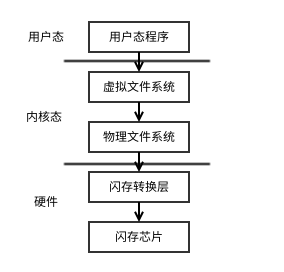
\includegraphics[width=0.4\textwidth]{traditional_ssd.png}}
    \hspace{4em}
    \subcaptionbox{开放通道SSD的访问流程\label{fig:imple_ocssd}}
        {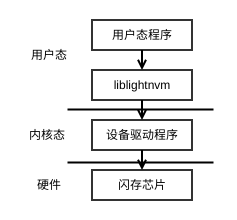
\includegraphics[width=0.4\textwidth]{ocssd.png}}
    \caption{两种SSD的访问流程}
    \label{fig:imple_ssdvisit}
\end{figure}

具体到本文的实现,为了便于评测时统计相关信息,实现时没有直接使用liblightnvm提供的读写接口,而是在开源的开放通道SSD评测工具fox的基础上进行改进。fox在liblightnvm提供的接口基础上增加了统计信息的记录,能够测量全过程的平均吞吐量,读/写/擦除操作的平均延迟以及精确到每页的读/写/擦除操作的大小和延迟。fox本身只提供了几种预先定义的IO序列,用于测试开放通道SSD的连续读取、连续写入和读取写入按一定比例混合交替进行时的性能。利用这些序列可以得到所用SSD的基本性能如表\ref{tab:imple_ocssd_perf}所示:

\begin{table}[htb]
    \centering
    \begin{minipage}[t]{0.8\linewidth}
    \caption{开放通道SSD的基本性能}
    \label{tab:imple_ocssd_perf}
      \begin{tabularx}{\linewidth}{YY}
        \toprule[1.5pt]
        {\heiti 操作} & {\heiti 延迟(单位us)} \\\midrule[1pt]
        读一个Page & 101\\
        写一个Page & 116\\
        擦除一个Block & 434\\
        \bottomrule[1.5pt]
    \end{tabularx}
\end{minipage}
\end{table}

由表\ref{tab:imple_ocssd_perf}可知,SSD的基本操作中擦除耗时远远高于读、写耗时,因此为高性能应用负载设计合适的优化策略时,应尽量避免过多的擦除操作和多余的写入操作。位于用户态的负载优化策略同样需要实现传统SSD的闪存转换层具有的地址映射、垃圾回收和负载均衡功能,因此下面从这三方面尝试设计较好的优化策略。

\section{映射方式}
\subsection{直接地址映射}
直接地址映射即不进行任何形式的逻辑地址到物理地址的转换,这一策略最为简单,但不适用于SSD设备。原因是SSD设备的写入以Page为单位,而擦除以Block为单位,且被写入后的页只有在所在块被擦除后才能重新写入。当负载中存在大量的覆盖写时,直接地址映射会要求被覆盖写的区域所在块被擦除后再写入新数据,同时未被覆盖的有效数据得到保留。这就增加了被覆盖写的块的擦除操作和重新写入有效数据的额外写操作,使得写入效率大幅下降。可行的做法是如非必要则不去真正清除被覆盖写的数据,而是将其标记为无效,同时在设备上为新写入的数据分配一块新空间。这种做法会导致同一个逻辑地址在多次写入时对应的物理地址发生变化,因此需要建立逻辑地址到物理地址的映射方式。
\subsection{页映射}

\subsection{超级块映射}

\section{垃圾回收策略}
\subsection{基于贪心原则的垃圾回收}
\subsection{连续空间上的垃圾回收}

\section{负载均衡}

\section{本章小结}